\documentclass[]{report}
\usepackage{graphicx}

% Title Page
\title{AR Mirror Game user manual}
\author{Tim van Rossum}


\begin{document}
\maketitle

\section*{Acquiring the source code}

The source code can be downloaded using git from the following repository:

\verb#git@github.com:thijser/ARGAME.git#

\section*{Building the server}

The server code is in the \verb#MirrorServer# directory and includes a Qt
Creator project to build it. It depends on the latest version of OpenCV, which
needs to be built manually using Visual Studio.

After building it, the "Projects" menu needs to be opened and the
\verb#OPENCV_HOME# variable needs to be set to a directory with the following
subdirectories:

\begin{itemize}
    \item \verb#include# - Include directories
    \item \verb#bin# - OpenCV DLLs
    \item \verb#lib# - OpenCV libraries
\end{itemize}

After running \verb#Build -> Run qmake# the server can then be built using
\verb#Build -> Rebuild All#. The output files will be placed in the \verb#dist#
folder in the repository root directory.

\section*{Starting up the server}
Before one can start up the server and actually have it do something, the master
camera needs to be connected to the computer that the server should run on. 
Then, the user should select whether completely red markers or red-and-yellow
markers should be detected as corner markers. They should also enter the camera
device ID (usually 1, if the computer has its own webcam, but it can also be 0.
It is advised to try out both options to find the one that works). The server
port and camera resolution can also be specified (the default server port is 
23369, and it is advised to not change it as that also has to be changed
client-side in that case). Enabling "Require empty board" will require the board
to be empty (no markers on the board) before the server is initialized. This is
used to capture an image of the empty board for remote players. \\
\\
The server UI also specifies some useful information: it shows the FPS the
server is recording the board at, the index of the current level, and a debug
overlay (if enabled) that shows what the camera sees, with marker indices
overlaid on the different markers. The server UI is shown in \ref{fig:serverui}
\begin{figure}[!ht]
    \centering
    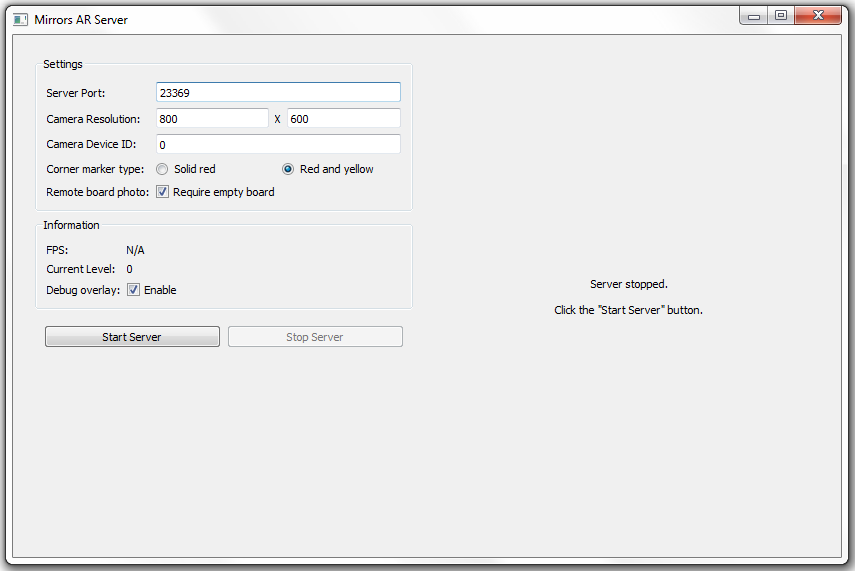
\includegraphics[scale = 0.5]{MirrorServerUI}
    \caption{The server UI.}
    \label{fig:serverui}
\end{figure}

\section*{Joining as a remote player}
In order to join the game as an extra remote player, one needs to have Unity
installed on their machine, as the interface for the remote player is a Unity
scene. The scene is called RemotePlayer.unity, and contains a single object,
the RemoteController object. This object contains a lot of scripts necessary
for the functioning of the remote player gameplay.\\
\\
In order to connect to the server, one has to know the IP address of the
device that the server runs on. Once known, the server can be accessed by
entering the IP address into the "Server Address" field of the Client Socket
component of the RemoteController object. The server port is set to a default
23369, and can be changed, but just like changing the port of the server,
this is not recommended. A detailed overview of the RemoteController object
and its options can be found in \ref{fig:remotecontroller}
\begin{figure}[!ht]
    \centering
    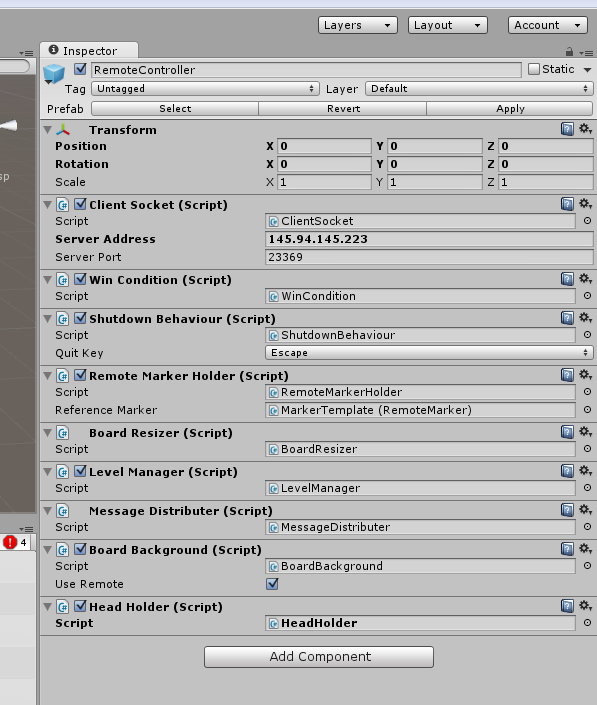
\includegraphics[scale = 0.6]{RemoteController}
    \caption{The settings for the RemoteController object.}
    \label{fig:remotecontroller}
\end{figure}

\section*{Joining as a local player}
In order to join the game as an extra local player one needs to have Unity
installed, just like with joining as an extra remote player, and to be able
to play properly as a local player, the player should also have a META One
connected to their device. The interface for the local player is also
a Unity scene. It contains a single object, the MetaWorld object. This object
contains all the settings necessary for the local player gameplay.\\
\\
In order to connect to the server, one has to know the IP address of the
device that the server runs on. Once known, the server can be accessed by
entering the IP address into the "Server Address" field of the Client Socket
component of the MetaWorld object. Again, it is possible to also change the
server port, but it is discouraged. The settings of the MetaWorld object
are shown in \ref{fig:metaworld}

\begin{figure}[!ht]
    \centering
    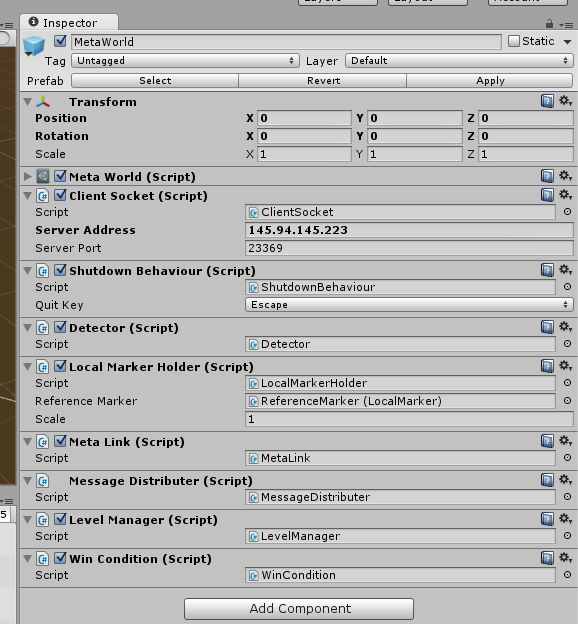
\includegraphics[scale = 0.6]{MetaWorld}
    \caption{The settings for the MetaWorld object.}
    \label{fig:metaworld}
\end{figure}

\end{document}          
